\documentclass[../main/main.tex]{subfiles}

\newdate{date}{29}{11}{2019}


\begin{document}



\chapter{Non ideal fluids: Mean field theory, Van der Walls, Virial expansion and Cluster expansion}

\marginpar{ \textbf{Lecture 14.} \\  \displaydate{date}. \\ Compiled:  \today.}

\section{Mean field theory for fluids}
Fluid system of \( N \) particles with position vectors \( \{ \va{r}_i \}_{i=1,\dots,N}   \). The configurational (grancanonical) partition function is (we can do Gaussian integrals)
\begin{equation}
  Q_N (T) = \int_{V}^{} \prod_{i=1}^{N}  \dd[]{\va{r}_i}  \exp [-\beta \Phi (\{ \va{r} \}  ) - \beta \sum_{i=1}^{N} \psi _{ext}  (\va{r}_i)]
\end{equation}
where \( \psi _{ext} \) is a one body potential, but we do not consider it because is not the aim of our problem.

In general,
\begin{equation}
  \Phi (\{ \va{r}_i \}  ) = \sum_{i,j>i}^{}  U_2 (\va{r}_i,\va{r}_j) + \sum_{i,j, \mu }^{} U_3 (\va{r}_i, \va{r}_j, \va{r}_ \mu ) + \dots
\end{equation}
but we forgot about \( U_3 \) that is the three body interaction.

 We consider
\begin{equation}
   U_2 (\va{r}_i,\va{r}_j) \rightarrow U_2 ( \abs{\va{r}_i - \va{r}_j} )
\end{equation}
Therefore,
\begin{equation}
  Q_N (T) = \int_{V}^{} \prod_{i=1}^{N}  \dd[]{\va{r}}  \exp [-\beta \sum_{i,j > i }^{}  U_2 ( \abs{\va{r}_i - \va{r}_j} ) ]
\end{equation}
Now, we replace all this story with just a field, it is a sort of average of the interactions. Doing the mean field assumption for \( U_2 \), we obtain
\begin{equation}
  \sum_{i,j > 1 }^{}  U_2 ( \abs{\va{r}_i - \va{r}_j} ) \rightarrow \sum_{i}^{} \Phi _{MF} (\va{r}_i)
\end{equation}

In particular, the \textbf{mean field approximation}  consists in substituting the multi-body interaction potential \(   \Phi (\{ \va{r}_i \}  ) \) with an effective one body potential \( \Phi (\va{r}) \) withing which all the particles move.
\begin{equation}
\Phi (\{ \va{r}_i \})   =\sum_{i}^{} \Phi _{MF} (\va{r}_i)
\end{equation}
As said, for simplicity consider \( \psi _{ext} = 0 \), hence
\begin{equation}
  Q_N (T) \simeq \qty[  \int_{V}^{} \prod_{i=1}^{N}  \dd[]{\va{r}}  \exp [-\beta \Phi _{MF} (\va{r})  ] ]^N
\end{equation}
\begin{remark}
The integral depends on the form of \( \Phi _{MF} (\va{r})  \).
\end{remark}
If one assumes the \emph{spatial isotropy},
what it is important is not anymore the vector but only the distance; hence, it is important just the integral over the modulus:
\begin{equation}
    \Phi _{MF} (\va{r}) = \Phi _{MF} (\abs{\va{r}} ) = \Phi _{MF} (r)
\end{equation}
In general
\begin{equation}
\Phi _{MF} (r) =
  \begin{cases}
   \infty & r < r_0 \quad  \text{repulsion}\\
   u < 0 & r> r_0  \quad \text{attraction}
  \end{cases}
\end{equation}
as plotted in Figure \ref{fig:14_1}.
\begin{figure}[h!]
\centering
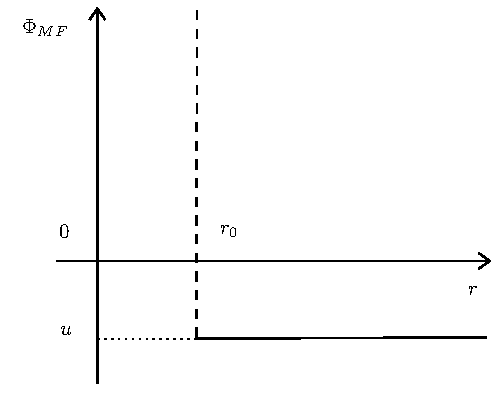
\includegraphics[width=0.6\textwidth]{../lessons/14_image/1.pdf}
\caption{\label{fig:14_1} Plot of the potential \( \Phi _{MF} (r) \).}
\end{figure}
Moreover,
\begin{equation}
  Q_N^{MF} (T) = \qty[ V_{ex}e^{- \infty } + (V-V_{ex})e^{-\beta u} ]^N
\end{equation}
where \( V_{ex} \simeq r_0^3 \) is the volume not accessible by the particle.
\begin{equation}
  Q_N^{MF} (T) = \qty[ (V-V_{ex})e^{-\beta u} ]^N
\end{equation}
The free energy is
\begin{equation}
  F_N^{MF} (T) = - N k_B T \qty[ \ln{(V-V_{ex})} - \beta u ]
\end{equation}
The pressure is
\begin{equation}
  P_N^{MF} = - \eval{\pdv{F_N^{MF}}{V} }_T = \frac{N k_B T}{V-V_{ex}} - N \qty(\pdv{u}{V} )_T
  \label{eq:14_1}
\end{equation}
\begin{remark}
In general, the deep \( u \)  can go up and down depending on the \emph{V}: \( u = u (V) \). This is becous \( u \) is the attractive well of the mean field potential and, for \( r \ge r_0 \) must be proportional to the fluid density
\begin{equation*}
  u \sim -N/V
\end{equation*}
where the minus sign means attraction. On the other hand, also \( V_{ex} \), the volume not accessible, must be proportional to \( N \),
\begin{equation*}
  V_{ex} = b N  \quad  \Rightarrow u = - a \frac{N}{V}
\end{equation*}
where \( b \) is the volume of a single particle.
\end{remark}
Inserting the last term in \eqref{eq:14_1}, we obtain the \emph{Van der Walls equation of state}:
\begin{equation}
  P_N^{MF} (V,T) = \frac{N k_B T}{V-bN} - a \qty(\frac{N}{V})^2
  \label{eq:14_2}
\end{equation}
\section{Equation of state and critical point}
Let us define the specific volume
\begin{equation}
  v \equiv \frac{1}{\rho } = \frac{V}{N}
\end{equation}
Hence,
\begin{equation}
P = \frac{K_B T}{v - b} - \frac{a}{v^2}
\end{equation}
We have this effect because it is a mean field, so the curve in Figure \ref{fig:14_2_1} it is replaced by the curve in Figure \ref{fig:14_2_2}.
\begin{figure}[h!]
\begin{minipage}[c]{0.5\linewidth}
\subfloat[][Description]{ 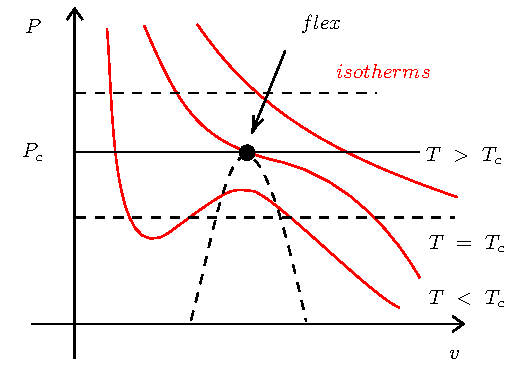
\includegraphics[width=0.9\textwidth]{../lessons/14_image/2.pdf}  \label{fig:14_2_1} }
\end{minipage}
\begin{minipage}[]{0.5\linewidth}
\centering
\subfloat[][Description]{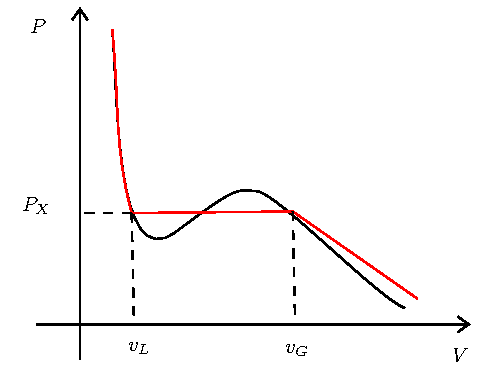
\includegraphics[width=0.9\textwidth]{../lessons/14_image/3.pdf}  \label{fig:14_2_2} }
\end{minipage}
\caption{\label{fig:} }
\end{figure}

For \( T < T_c \) the equation \( P(v) = const \) has 3 distinct solutions. For \( T > T_c \) only one solution \( \in \R \).

\begin{itemize}
\item
The \emph{inflection point condition} at \( T = T_c \) is
\begin{equation}
  \pdv{P}{v} = \pdv[2]{P}{v} = 0
\end{equation}
and these are the critical point conditions. The second in particular means that there is a flex point. Let us pay attention to it, indeed it is a standard way to find critical points.
We obtain  \( v_c = 3 b \):
\begin{equation}
  P_c = \frac{a}{27 b^2}, \quad k_B T_c = \frac{8a}{27b}
\end{equation}
and
\begin{equation}
  \frac{P_c v_c}{k_B T_c} = \frac{3}{8}  \approx 0.375
\end{equation}

\item Another way to find the critical point consists in noticing that at \( T=T_c \), the 3 solutions coincide.
Let us rewrite the equation of state
\begin{equation}
  P = \frac{v^2 k_B T - a (v-b)}{v^2 (v-b)}
\end{equation}
as
\begin{equation}
  v^3 - \qty(b + \frac{k_B T}{P})v^2 + \frac{a}{P} v - \frac{a b }{P} = 0
  \label{eq:14_3}
\end{equation}
Since at \( T=T_c \) the 3 solutions coincide, equation  \eqref{eq:14_3} must be of the form
\begin{equation}
  (v-v_c)^3 = 0 \quad \Rightarrow v^3 - 3 v^2 v_c + 3 v v_c^2 - v_c^3 = 0
\end{equation}
and, by identifying its coefficients with the ones in \eqref{eq:14_3} one gets
\begin{equation}
  v_c^3 = \frac{a b}{P_c}, \quad 3 v_c^2 = \frac{a}{P_c}, \quad 3 v_c = b + \frac{k_B T_c}{P_c}
\end{equation}
Giving
\begin{equation}
  v_c = 3 b, \quad P_c = \frac{a}{27 b^2}, \quad k_B T_c = \frac{8 a }{27 b }
  \label{eq:14_4}
\end{equation}
From the relations \eqref{eq:14_4}, it is clear that it is sufficient to estimate the \( a \) and \( b \) coefficients of a gas using the equation of state at \( T \) sufficiently high to estimate its critical values, \( v_c \), \( T_c \) and \( P_c \).
Moreover, one can show that
\begin{equation}
    \frac{P_c v_c}{k_B T_c} = \frac{3}{8}  \approx 0.375
\end{equation}
It is an universal ratio whose value does not depends on either \( a \) or \( b \).
\end{itemize}

\subsection{Law of the correspondent states}
The universal value of the ratio \( \frac{P_c v_c}{k_B T_c} \) suggests a deeper correspondence between different fluid systems.

Let us rewrite the Van der Walls equation of state \eqref{eq:14_2} in adimensional form
\begin{equation}
  \pi \equiv \frac{P}{P_c}, \quad \nu  \equiv \frac{v}{v_c}, \quad \tau \equiv \frac{T}{T_c}
\end{equation}
The result is
\begin{equation}
  \qty(\pi + \frac{3}{\nu ^2}) \qty(3 \nu -1) = 8 \tau
\end{equation}
\begin{remark}
When rescaled by \( P_c, v_c \) and \( T_c \), the thermodynamic variables \( P,v \) and \( T \) of the Van der Walls fluids, follow the same equation of state! The Van der Walls theory describes the law of correspondent states found experimentally.
\end{remark}

\section{Region of coexistence and Maxwell construction}
In real fluids, for \( T < T_c \) \( (\tau < 1) \), there is a first order liquid-gas transition with coexistence between vapor and liquid phase and non analiticity of the thermodynamic potential. In particular, an isotherm for \( T < T_c \) is the one in Figure \ref{fig:14_2_2}. How this is described by the mean-field (i.e. Van der Walls) theory?   




\section{lesson}


Try to do the expansion around the critical point, \( t = \tau -1 = \frac{T-T_c}{T_c}\) and \( \Phi = \nu -1 = \frac{v-v_c}{v_c} \). You want the deviation from the critical point.


\begin{equation}
  Q_N (T) = \int_{V}^{} \prod_{i=1}^{N}  \dd[]{\va{r}}  \exp [-\beta \sum_{i,j > i }^{}  U_2 ( \abs{\va{r}_i - \va{r}_j} ) ]
\end{equation}

\begin{equation}
  Z_N = \frac{1}{N! \Lambda ^{3N} } Q_N
\end{equation}
For an ideal gas we have: \( Q_N = V^N \)
\begin{equation}
  \rightarrow Z_N^{ideal} = \frac{V^N}{N! \Lambda ^{3N}}
\end{equation}
Now, suppose that \( U_2 \neq 0  \) but small! We can say that we can assume that our \( Q_N (V,T) \) it would be the ideal version times a new function
\begin{equation}
  Q_N (V,T)=V^N \chi _N (V,T)
\end{equation}
so
\begin{equation}
  F_N = F_N^{ideal} - k_B T \ln{\chi _N}
\end{equation}
This also suggest, that you can formally expand the equation of state as a function of the density
\begin{equation}
  \frac{P}{k_B T} = \rho
\end{equation}
this is the ideal gas, now start to add the other terms of the expansion
\begin{equation}
  \rightarrow \frac{P}{k_B T} = \rho + B_2 (T) \rho ^2 + B_3 (T)\rho ^3+ \dots + O(\rho ^n)
\end{equation}
this is a \emph{virial expansion}, it is one of the most used. The coefficient \( B \) are called the \emph{virial coefficients}.  Making a fit, you will obtain the virial coefficients. This is what physicist have done for years. Mapping the coefficient with the real world experiments, you can find some macroscopical parameters.

\begin{equation}
  \frac{P}{k_B T} = \frac{N}{V-bN} - \frac{a N^2}{k_B T V^2}
\end{equation}
do an expansion, you will get the same structure of the virial expansion, finding the virial coefficient of the Van der Walls. Therefore,
\begin{equation}
  B_2 (T)^{VdW} = b - \frac{a}{k_B T} \qquad B_3^{VdW} = b^2
\end{equation}
The \emph{Boyle's temperature} is when the second coefficient is zero:
\begin{equation}
  B_2^{VdW} (T_B) = 0
\end{equation}
so you remove the most important coefficient.
We have \( T_B \) versus \( T_c \). It is clear that the Boyle's temperature must be much greater than the critical one. Consider a polymer, the transition point called the \( \theta  \) point is when the second coefficient is zero, as the case described above, but it is interesting in polymer kind of system.

Let us try to do some calculation of this virial coefficients, starting from the model microscopical
\begin{equation}
  Q_N = \int_{V}^{} \dd[]{\va{r}_1} \dots \int_{V}^{} \dd[]{\va{r}_N}  e^{-\beta \sum_{i,j > i}^{} \Phi _{ij} }
\end{equation}
with
\begin{equation}
  \Phi _{ij} = \Phi ( \abs{\va{r}_i - \va{r}_j} )
\end{equation}
The \emph{Mayer function}  is something that is smaller in that given point
\begin{equation}
  f (\abs{\va{r}} ) \equiv \exp [ - \beta \Phi ( \abs{\va{r}} )] -1
\end{equation}
If \( \beta \Phi \ll 1 \), we have \( f \ll 1 \). So
\begin{equation}
  \rightarrow  e^{-\beta \sum_{i,j > i}^{} \Phi _{ij} } = \prod_{i}^{} \qty(\prod_{j>i}^{} (1+ f_{ij})  )
\end{equation}
Expanding this object we obtain
\begin{equation}
  \rightarrow = \underbrace{(1+f_{12})(1+f_{13}) (1+ f_{14}) \dots ( 1 + f_{1N })}_{i=1}   \dots \underbrace{(1+f_{23}) (1+ f_{24}) \dots ( 1 + f_{2N })}_{i=2} \dots =
\end{equation}
\begin{equation}
  = 1 + \sum_{i}^{} \sum_{j>i}^{} f_{ij} + \cancel{\sum_{i}^{} \sum_{k \ge i}^{} \sum_{j > i}^{} \sum_{e \ge j}^{} f_{ik} f_{je}       }
\end{equation}
The solution is given by considering only the linear term. This is the cluster expansion.



\end{document}
